\chapter{Optimization}

In optimization the goal is to optimize a performance measure. Ideally we should aim to optimize the true error but in Machine Learning the true error is not computable.

$$J(\theta) = \mathbb{E}_{(x, y) \sim S} L(f(x, \theta), y) = \frac{1}{n} \sum_{i=1}^{n} L(f(x^{(i)}, \theta), y^{(i)})$$

where S is the sample data that we have in our dataset. If the sample size is large enough the true error and the empirical error are approximately the same. However, this approach can lead to overfitting, where the model memorizes the training data rather than generalizing. Additionally, many loss functions used in deep learning are not differentiable (e.g. 0-1 Loss), making it difficult to employ gradient descent. Therefore, we will require specialized techniques and novel approaches to effectively train neural networks such as using a surrogate loss (e.g. negative log likelihood as surrogate for 0-1 loss) that can be used together with gradient descent.

\section{Batch/Mini-batch Algorithms}

A common optimization technique are the the batch/mini-batch algorithms. These are divided depending on the amount of the original data that we use.

\begin{itemize}
    \item Batch or Deterministic Gradient Descent: This algorithm computes the gradient of the loss on the whole training set and then updates the weights. Therefore it has the advantage of computing the right gradient but on the other hand it will be very costly and slow. It will also only update the weights one time per epoch.
    \item Online or Stochastic Gradient Descent: This algorithm computes the gradient of the loss on a single sample on the training set and then updates the weights. This has the advantage of performing a weight update once per sample (we will do n updates per epoch where n is the data size). On the other hand, the gradient is less accurate since it computes the gradient of the loss only with respect to a single example.
    \item Mini-batch Stochastic Gradient Descent: This algorithm is a compromise between the last two methods. It computes the gradient of the Loss on a subset of examples (mini-batch) of the training set and then updates the weights. This approach provides a compromise between the accurate gradient computation of batch gradient descent and the increased number of weight updates of stochastic gradient descent.    
\end{itemize}

\noindent Overall this technique reduces the computational cost and has a regularization effect (noise in the gradient). Therefore, the algorithm will converge faster at the expense of using less accurate gradient estimations with respect to the exact gradient.

\newpage

\section{Challenges in Optimization}

The most prominent challenges involved in optimization for training deep models are:

\subsection{Ill-Conditioning of Hessian}

Ill-conditioning of the Hessian matrix occurs when the second derivatives have a large variance, making it difficult for first-order methods like Stochastic Gradient Descent to converge. If the function to optimize resembles a long canyon (the direction with most curvature has way more curvature than the direction with the least curvature) there will be an inefficient zigzagging while performing the SGD algorithm which wastes time and slows down the convergence of the optimization algorithm.

\begin{figure}[h]
    \centering
    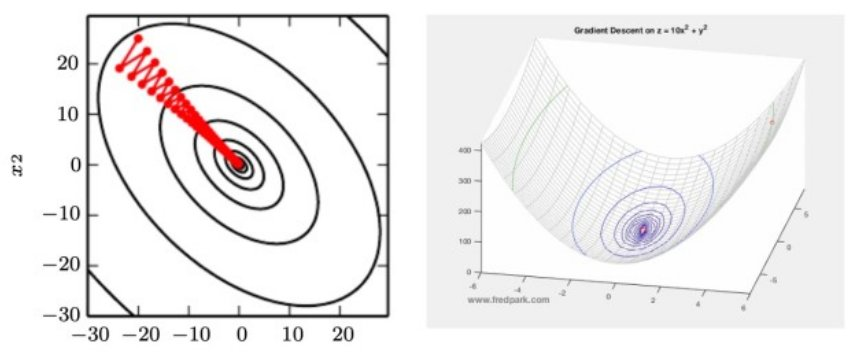
\includegraphics[width=10cm]{Plots/ill-conditioned-hessian.jpg}
    \caption{Zig-zagging of the gradient in a ill conditioned Hessian}
\end{figure}

\subsection{Saddle Points and Local Minima}

Because in Neural Networks training we are dealing with a non-convex cost function we will have many non-optimal local minima due to symmetries and weight scaling. In the past this used to be considered a major problem in Deep Learning but nowadays is has been shown that  it is sufficient to find a point with low cost as different parameter configurations can achieve similar performance. Additionally, in high-dimensional spaces, saddle points are more common than local minima. This is because saddle points have a mix of positive and negative eigenvalues in their Hessian matrix, while local minima have only positive eigenvalues. In a n-dimensional space it is exponentially unlikely that all eigenvalues are positive.

\begin{figure}[h]
    \centering
    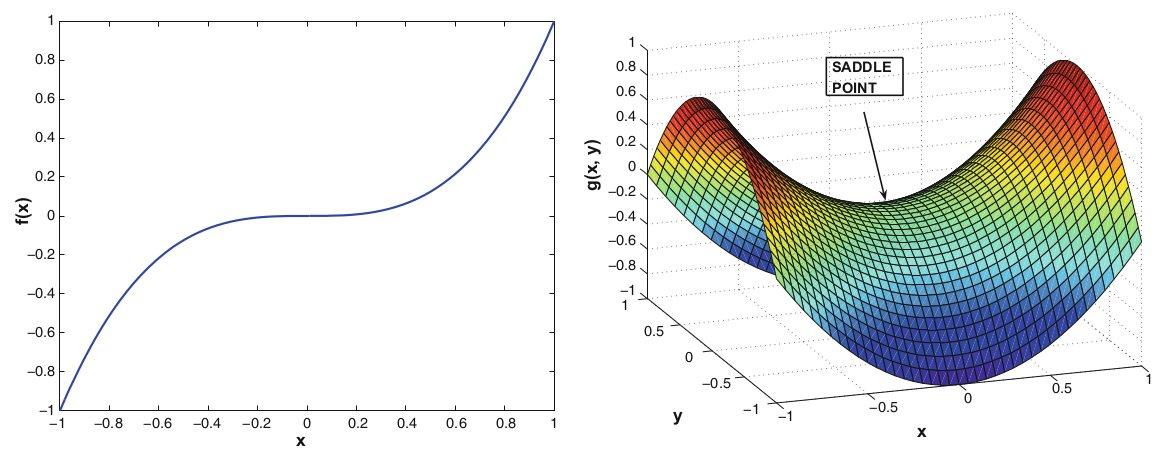
\includegraphics[width=10cm]{Plots/saddle-point.jpg}
    \caption{Example of 1 dimensional and 2 dimensional saddle points.}
\end{figure}

\noindent Saddle points can also pose challenges for optimization algorithms. First-order methods like Stochastic Gradient Descent has proven to be able to escape saddle points quickly due to the small gradient near them. In contrast, second-order methods may jump to saddle points. This is why first-order methods are preferred for training deep neural networks.

\newpage

\subsection{Flat Regions}

Flat regions, where both the gradient and the Hessian are close to zero, makes it difficult for the algorithm to determine the direction of improvement and navigate towards better solutions.

\begin{figure}[h]
    \centering
    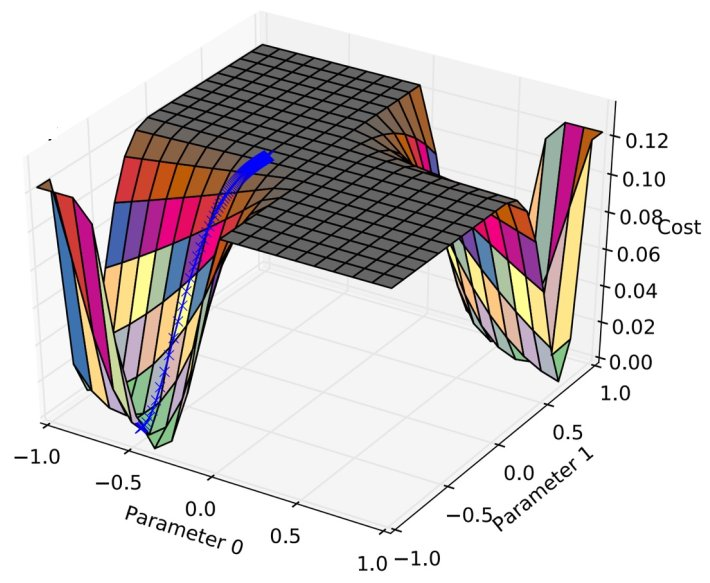
\includegraphics[width=6.5cm]{Plots/flat-regions.jpg}
    \caption{Example of a 2 dimensional flat region}
\end{figure}

\subsection{Cliffs and Exploding Gradients}

Deep Neural Networks may have extremely steep regions called cliffs which cause the gradient to become large, resulting in weight updates that jump far away. To mitigate the issues caused by exploding gradients and the instability they introduce, a technique called gradient clipping is often employed. This one consists in limiting the magnitude of the gradient, preventing it from growing too large. By reducing the step size, gradient clipping helps stabilize the training process and prevents weight updates from taking excessively large leaps.

\begin{figure}[h]
    \centering
    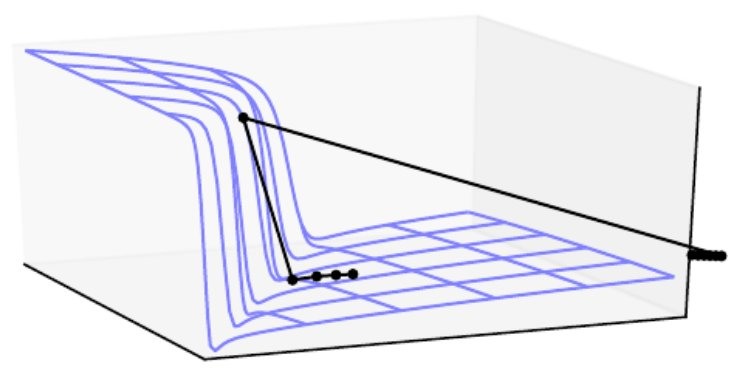
\includegraphics[width=6.5cm]{Plots/cliffs.jpg}
    \caption{Example of a cliff in gradients}
    \label{fig:gradient-cliff}
\end{figure}

\subsection{Exploding/Vanishing Gradients}

Another problematic challenge is the issue of exploding and vanishing gradients. This happens in Recurrent Neural Networks due to repeatedly multiply the input by the weight matrix $W$.

$$ W = V diag(\lambda) V^{-1} $$

\noindent Multiplying this matrix $t$ times we end up with.

$$W^{t} = V {diag(\lambda)}^t V^{-1}$$

\noindent If the eigenvalues are not close to 1, they will either vanish (eigenvalues << 1) or explode (eigenvalues >> 1). Cliffs are an example of exploding gradients.

\noindent We will have a similar problem with activation functions that can saturate (e.g sigmoid) which will produce a vanishing gradient. However, feed-forward networks with non-saturating activation functions, like ReLU, and different matrices for each layer, avoid this problem.

\newpage

\section{Stochastic Gradient Descent}

Stochastic Gradient Descent is a variation of Gradient Descent that makes use of a mini-batch m to compute the gradient instead of the whole dataset (making it less computationally expensive). This introduces noise which makes the algorithm more able to escape from local minimum and saddle points. Therefore, Stochastic Gradient Descent is in general a more robust algorithm and can reach better solutions compared with vanilla Gradient Descent. Another difference is that we have an adaptative learning rate $\eta$. The Stochastic Gradient Descent algorithm updates the $W$ parameters of layer $l$ as follows:

$$ W_{t+1}^{l} = W_{t}^{l} - \eta \frac{\partial J}{\partial W_{t}^{l}} $$

\subsection{Momentum}

Stochastic Gradient Descent can be slow, so in order to speed up the training a momentum is introduced. Momentum therefore helps accelerate convergence, especially in cases where the loss landscape has irregularities or noisy gradients. The Stochastic Gradient Descent algorithm with momentum is as follows:

$$ v = \beta v - \eta \frac{\partial J}{\partial W_{t}^{l}}  ~~~  W_{t+1}^{l} = W_{t}^{l} + v $$

\noindent The momentum is initialized at 0 since at the beginning of the optimization process, there is no accumulated momentum from previous iterations. The momentum term $\beta$ is a value between 0 and 1 (usually is set to 0.9). 

Introducing momentum produces that the gradient in one direction is increased if all these gradients are aligned over multiple iterations but decreased if the gradient direction repeatedly changes. The overall effect is a smoother trajectory and reduced oscillatory behavior in valleys making the algorithm able to navigate noisy or small gradients more efficiently, leading to faster convergence.

\subsection{Nesterov Momentum}

Another optimization algorithm that introduces a variance of momentum is called the Nesterov momentum. The Stochastic Gradient Descent algorithm is now:

$$ \tilde{W}_{t}^{l} = W_{t}^{l} + v $$

$$ v = \beta v - \eta \frac{\partial J}{\partial \tilde{W}_{t}^{l}}  ~~~~~  W_{t+1}^{l} = W_{t}^{l} + v $$

\noindent In Nesterov momentum the gradient is evaluated after the current velocity is applied. Thus one can interpret Nesterov momentum as attempting to add a correction factor to the standard method of momentum.

\section{Parameter Initialization}

Parameter initialization is a crucial step on our Deep Neural Network models as these ones are very dependent on the initialization points. Bad initial points can cause numerical instabilities and algorithm failure. In the general case where various activation functions like sigmoid or tanh are used, initializing all weights to zero is problematic because it leads to the symmetry problem. Basically, when all weights in a layer are the same, neurons compute identical functions and they will evolve into the same values, resulting in redundant behavior. The layer will be equivalent to a layer with only one neuron. Breaking symmetry with proper initialization ensures stable training and a better generalization.

\noindent On the other hand, when using the ReLU activation function, although this one avoids the symmetry problem, initializing all weights to zero is neither a a good idea. In a network with ReLU activations, neurons with zero weights (or weights that become zero after initialization) will always output zero for any input during forward propagation. This leads to the problem of "dead neurons". Dead neurons cannot recover during training because their gradients are always zero (due to the ReLU derivative being zero for negative inputs). Having a significant number of dead neurons can severely limit the expressive power of the network and lead to suboptimal performance. It essentially reduces the network's capacity to represent complex functions and patterns in the data.

A common strategy is to initialize the weights randomly taking the values from a Gaussian or uniform distribution. Keep in mind that large weights can cause issues like exploding values or gradient saturation. Therefore, it is common to initialize weights close to zero with a specific scale. For fully connected layers with m inputs and n outputs heuristics like the uniform distribution are used.

$$ W_{i, j} \sim U \left(  \frac{-1}{\sqrt{m}}, \frac{1}{\sqrt{m}} \right) $$


\noindent Biases are often initialized with pre-defined constants to avoid saturation (usually 0 or 0.1 for ReLU to avoid saturation).

\section{Algorithms with Adaptative Learning Rates}

Gradient Descent algorithm with a fixed step size has an undesirable property: it makes large adjustments to parameters associated with large gradients and small adjustments to parameters associated with small gradients. A number of mini-batch-based algorithms have been introduced that adapt the learning rates of model parameters.

\subsection{AdaGrad}

AdaGrad is an optimization algorithm that scales learning rates inversely proportional to the square root of the sum of all of their historical squared values. The parameters with the largest partial derivative of the loss have a correspondingly rapid decrease in their learning rate, while parameters with small partial derivatives have a relatively small decrease in their learning rate. The net effect is greater progress in the more gently sloped directions of parameter space.

\noindent We update the accumulator as:

$$ G_{t}^{l} = G_{t-1}^{l} + \left( \frac{\partial J}{\partial W_{t}^{l}}  \right)^2  $$

\noindent Update the weights:

$$ W_{t+1}^{l} = W_{t}^{l} - \frac{\eta}{\sqrt{G_{t}^{l} + \delta}} \frac{\partial J}{\partial W_{t}^{l}} $$

\subsection{RMSProp}

In AdaGrad, the accumulation from the beginning of the training results in an excessive decrease in the learning rate. The RMSProp algorithm modifies AdaGrad to solve this issue by changing the gradient accumulation into an exponentially weighted moving average. The idea is to only converge rapidly after finding a convex bowl.

\noindent We update the accumulator as:

$$ G_{t}^{l} = \beta G_{t-1}^{l} + (1 - \beta) \left( \frac{\partial J}{\partial W_{t}^{l}}  \right)^2  $$

\noindent Update the weights:

$$ W_{t+1}^{l} = W_{t}^{l} - \frac{\eta}{\sqrt{G_{t}^{l} + \delta}} \frac{\partial J}{\partial W_{t}^{l}} $$


\subsection{Adam}

Adam combines the benefits of both the AdaGrad algorithm and RMSprop. Adam maintains adaptive learning rates for individual parameters by using estimates of first and second moments of the gradients:

\noindent We update the biased first moment estimate as:

$$ s = \beta_{1}s + (1 - \beta_{1})\frac{\partial J}{\partial W_{t}^{l}} $$

\noindent We update the biased second moment estimate as:

$$ r = \beta_{2}r + (1 - \beta_{2})\left( \frac{\partial J}{\partial W_{t}^{l}}  \right)^2 $$

\noindent Correct the bias in the first moment:

$$ \tilde{s} = \frac{s}{1 - \beta_{1}^{t}} $$

\noindent Correct the bias in the second moment:

$$ \tilde{r} = \frac{r}{1 - \beta_{2}^{t}} $$

\noindent Update the weights:

$$ W_{t+1}^{l} = W_{t}^{l} -\eta \frac{\tilde{s}}{\sqrt{\tilde{r}} + \delta}   $$


where $\beta_{1}$ and $\beta_{2}$ are the exponential decay rates for moment estimates. Usually their values are 0.9 and 0.999 respectively. Meanwhile $\delta$ is used for numerical stabilization. An often used value for this parameter is $10^{-8}$.

\section{Second Order Methods}

For now we have only seen first-order methods (e.g. SGD) for training Neural Networks. Second-order methods that consider curvature can perform better but are computationally expensive due to Hessian matrix computation.

\subsection{Newton's Method}

Newton's method is a second-order optimization algorithm, which means it uses not only the gradient but also the Hessian matrix. Consider the empirical risk as:

$$ J(\theta) = \frac{1}{n} \sum_{i=1}^n L \left( f \left( h^{(i)}, \theta \right) , y^{(i)} \right) $$

\newpage
\noindent and the the second-order Taylor series

$$ J(\theta + \delta) = J(\theta) + \delta^T \nabla_{\theta} J(\theta) + \frac{1}{2} \delta^T H(\theta) \delta $$

\noindent Newton method finds the optimal update step value for $\delta$ to minimize the cost function $J(\theta)$.

$$ \frac{\partial J(\theta + \delta)}{\partial \delta} = \nabla_{\theta} J(\theta) + H(\theta) \delta = 0 ~~~~~ \rightarrow ~~~~~ \delta^{"*"} = H^{-1} (\theta) \nabla_{\theta} J(\theta_0) $$

\noindent Computing $H$ and $H^{-1}$ is computationally unfeasible for ven medium size networks. 




